\section{Hydra Operational Details} \label{sec:data-operations}

To demonstrate how Hydra performs data operations, we will utilize an initial deployment on FABRIC\cite{}.

For the scenario, all of the following FABRIC sites have a Hydra node:
\begin{itemize}
    \item Clemson
    \item StarLight
    \item Washington
    \item Dallas
    \item Salt Lake City
    \item San Diego
\end{itemize}

\jcp{talk about the command table}

Imagine the scenario where Clemson's Genomics and Bioinformatics facility decides to use Hydra to store pre-processed (i.e. indexed) genomes. The main goal of this exercise is to allow data access for the researchers and their collaborators in a reliable manner.
%for themselves and others to use this data without spending valuable resources on the genome indexing pre-processing step. 

A user can download the correct set of files and insert into downstream analytic workflows simply by asking for these datasets by name. \jcp{why does the user care about this?}

%Hydra will dramatically simplify data processing. Of course, they are able to re-process the raw genome data files if needed.

\subsection{User Bootstrapping - Tianyuan}
\label{sec:dataop-bootstrap}
In order to bootstrap a Hydra user into the system, each Hydra user needs to obtain trust anchor, trust policies of Hydra and and get certified by the Hydra NOC

In Hydra, each user obtains the Hydra trust anchor and initial trust policies out-of-band.
After that, Hydra NOC authenticates each user on their email addresses.
This requires Hydra NOC knowing trustworthy email addresses via initial out-of-band trust relations.
We rely on the human trust relations between users and the NOC operator to realize the user authentication. 
The NOC operator maintains a list of trustworthy email addresses and configures the it to the NOC application.

Hydra user utilizes NDNCERT~\cite{} to perform the email authentication and obtains certificate from NOC.
Specifically, Hydra NOC as the NDNCERT CA does the following steps upon receiving a certificate request from a Hydra user.
It first checks the Hydra user email address membership, then verifies the email address by sending a PIN and requesting sending back in NDNCERT message.
Upon successful email membership and possession verification, Hydra NOC uses the user naming convention\ty{where's the user naming convention?} to assign the user an NDN name based on its email and certifies it.

As the final step, a Hydra user completes its security bootstrapping by obtaining and installing the issued certificate.

\subsection{Data Insertion} \label{sec:data-insert}

\subsubsection{Scenario}
Alice, a graduate student who is doing research at the Clemson's Genomics and Bioinformatics facility, has produced a pre-processed (i.e. indexed) axolotl genome that she believes is critical in understanding an axolotl's ability to regenerate tissue. She desires to publish this data in the form of a File within Hydra. To satisfy this scenario, she performs the following interactions with Hydra.


\subsubsection{User-to-Node Interaction}
\begin{figure}[!ht]
    \centering
    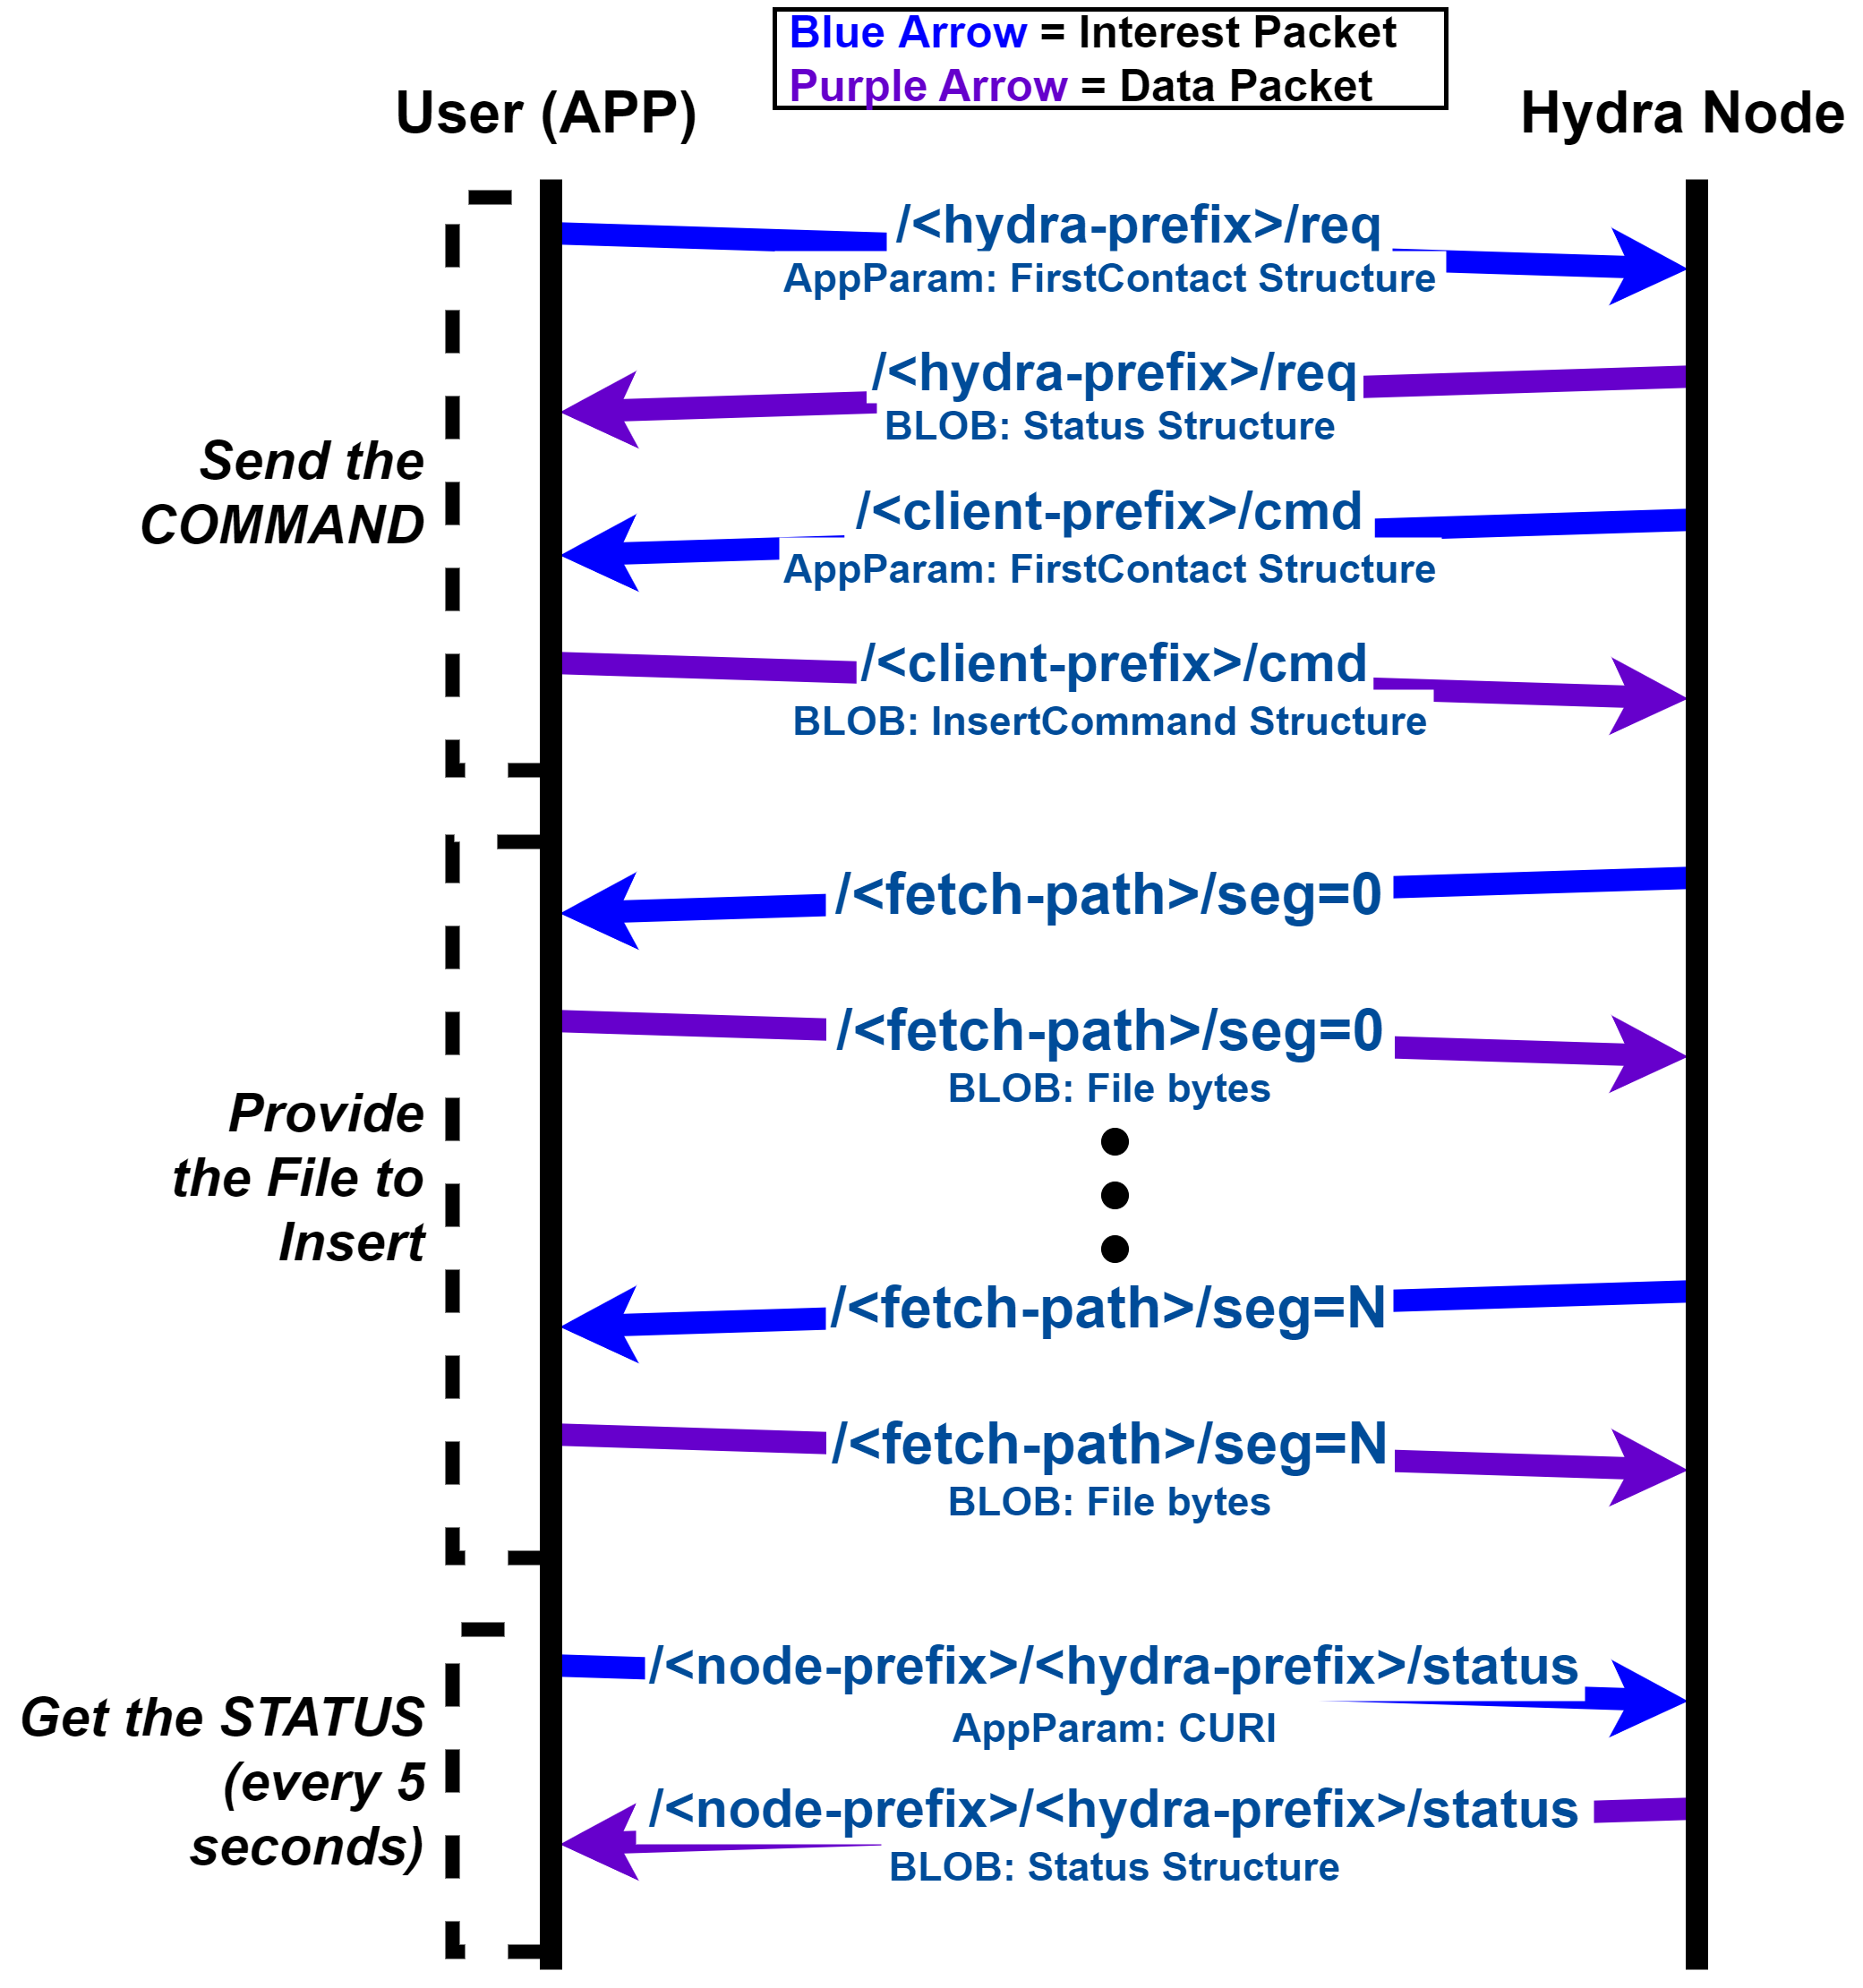
\includegraphics[width=\columnwidth]{visuals/insert-usr.png}
    \caption{NDN Interaction of A User and A Hydra Node During Data Insertion}
    \label{fig:insert-usr}
\end{figure}

The process of how a user will interact with a Hydra node via NDN is described in Figure~\ref{fig:insert-usr}. Any Hydra node can be contacted by the user for data insertion, and this interaction can be summarized as a PubSub-like interaction: it uses a notification Interest with a component /notify and data retrieval via /msg.
\todo[inline]{Define first contact structure and give and example}
\todo[inline]{user authentication is missing}
\xw{how to authenticate}
This interaction between user (A) and node (X) goes as follows:
\begin{enumerate}
    \item User (A) will send an Interest notification using the prefix /<hydra-prefix/insert, announcing that it has a command for any Hydra node to process.
    \item Upon hearing this, node (X) will send an Interest to fetch this command using user (A)'s prefix (stated in user (A)'s FirstContact structure found in the Interest notification's app parameters).
    \item Node (X) will begin to process this command; and because the command is an insertion, node (X) will begin to fetch file (F) using user (A)'s fetch path (found in the InsertCommand structure).
    \item Once file (F) is retrieved, node (X) will send a notification Interest stating that the command that user (a) sent has a updated status.
    \item User (A) can then fetch the status of the command using node (X)'s prefix (stated in node (X)'s FirstContact structure found in a previous interest).
\end{enumerate}

There are a few key points throughout this process.
\begin{enumerate}
    \item User (A) can fetch the status at any time as it has the necessary info; however if the command is not ready, node (X) will tell user (A) to wait. This is particularly useful in case node (X) goes offline. \todo[inline]{if X goes offline, how does it tell the user?}
    \item The switch from anycast to unicast is necessary to ensure a proper response as command information is not directly shared between Hydra nodes.
    \item Throughout the interaction, a command unique resource identifier (curi) is used. This allows Hydra nodes to process more than one command from a user and allows users to send more than one command.
    \todo[inline]{example of curi}
\end{enumerate}


\subsubsection{Module Interaction}
\begin{figure}[!ht]
    \centering
    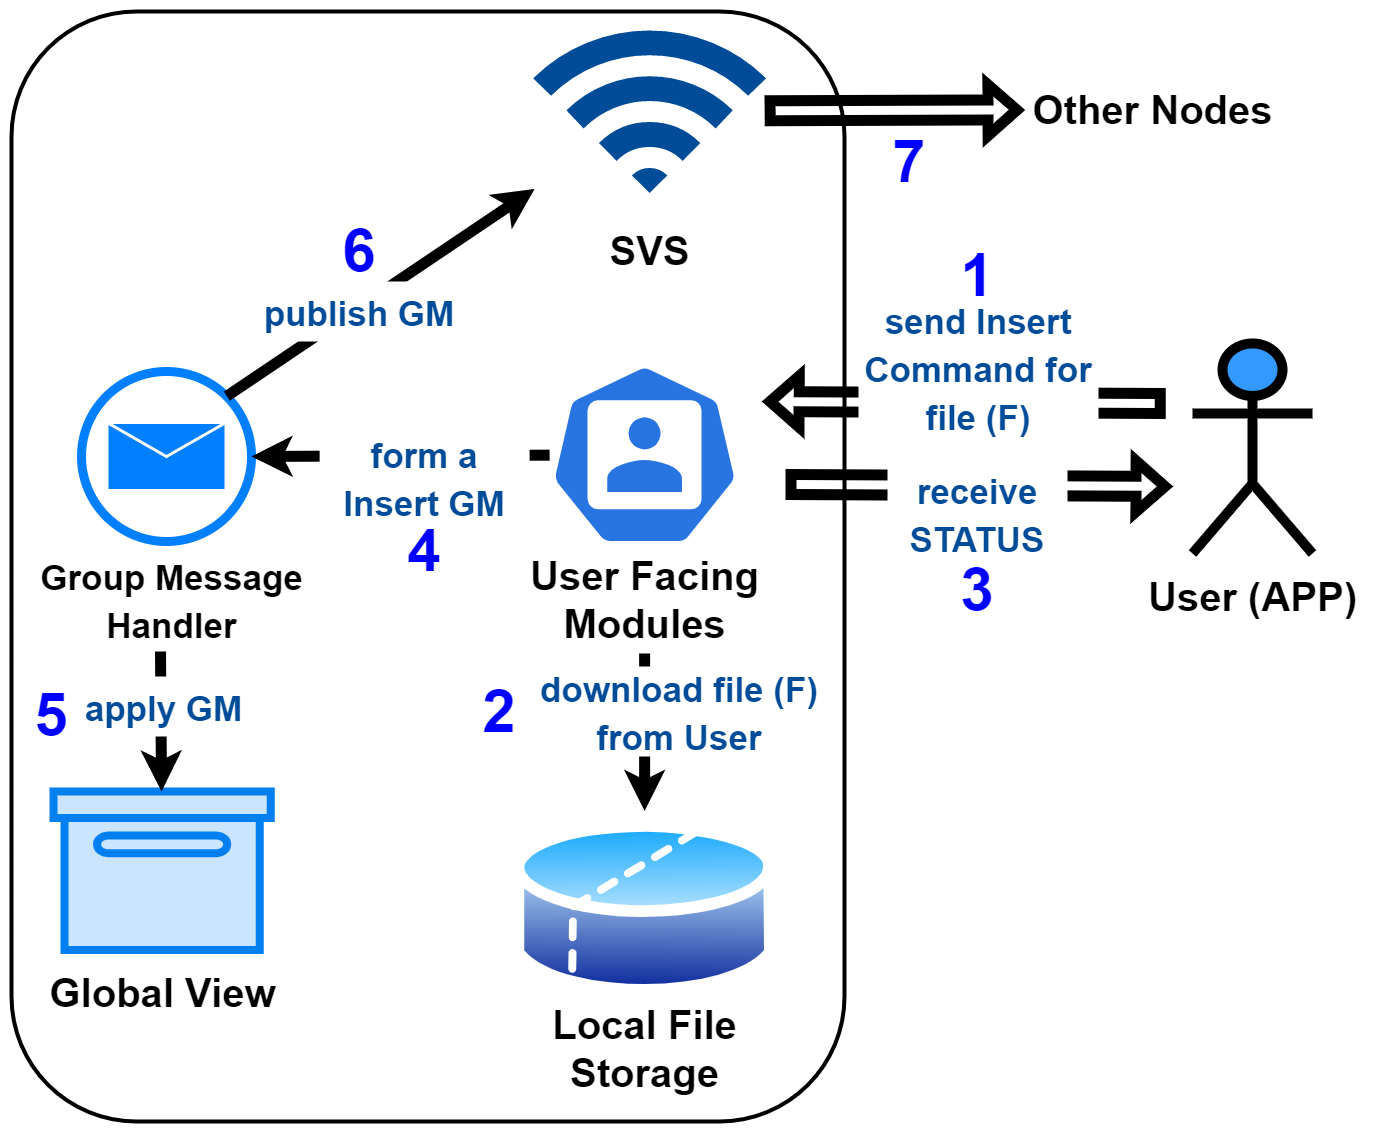
\includegraphics[width=\columnwidth]{visuals/insert-sys.png}
    \caption{Module Interaction to Fulfill a User's Insertion Command}
    \label{fig:insert-sys}
\end{figure}

The User-to-Node interaction leads to several interactions within Hydra.% node will act out the given command. 
Figure~\ref{fig:insert-sys} shows these interactions. When node (X) receives an Insertion command for file (F) from user (A):
\begin{enumerate}
    \item Node (X) properly authenticates the command, checks to see if the command can be executed, and then immediately starts fetching file (F) if the command satisfies all requirements.
    \item After storing file (F), node (X) updates the status for user (A) allowing user (A) to go offline.
    \item Node (X) then forms an Insert GM which includes all file metadata such as file name, size, etc. and states that node (X) will be storing this file.
    \item Node (X) applies this GM to its Global View.
    \item Node (X) publishes this GM using SVS, our distributed synchronization protocol.
\end{enumerate}

Every node will receive the Insert GM. When node (Y) receives the Insert GM sent by node (X) containing file (F)'s info, it performs the following operations:
\begin{enumerate}
    \item Node (Y) applies the GM to its Global View: file (F) information is added.
    \item Node (Y) sees that there is a replication need as file (F) does not meet the replication degree of 3 (stated in Hydra's base policy). For how replication is done, see Subsection~\ref{sec:data-replicate}
\end{enumerate}

\subsubsection{Data Structure Formats}
There are several structures that are used for the entire data insertion process. For the group message structures used in Module interaction, please refer back to Section~\ref{sec:group-messages}.

The structures used in User-to-Node interaction include the following:
\begin{enumerate}
    \item FirstContact: This includes the preferred name prefix that the sender wants to use for further interaction and a sender command unique resource identifier (curi) that the sender will use to refer to this interaction.
    \item InsertCommand: This include all necessary info that a Hydra node needs for a publication which includes a fetch path, file name, and other metainfo about the file.
    \item NotificationSpecification: This simply includes a command unique resource identifier (curi) of the receiver that the sender is referring to.
    \item CommandStatus: This just contains a Status code that can give simple feedback to the user. Theses codes are very simple and based on HTTP response status codes, please see Table \ref{tab:status-codes}. %\todo[inline]{define the status codes}
\end{enumerate}
\subsection{Data Replication - Justin} \label{sec:data-replicate}


\subsubsection{Scenario}
The FABRIC platform that the Hydra instance is running on is seeing a dramatic increase in popularity. As such, new sites have been installed and more users have been added. With tens of sites and users, site failures can happen.
%occurrence like in most distributed systems. However, there can be temporary outages as well that FABRIC experiences. Therefore, 
Hydra needs to have a fast replication mechanism in order to quickly recover from Hydra node failures.
%while also making temporary outages not as expensive. Also, 
Hydra should be able to copy Alice's file that she inserted in Subsection~\ref{sec:data-insert} several times (3 being Hydra's base policy) to prevent permanent file loss. To satisfy these scenarios, the following interactions are conducted.


\subsubsection{Module Interaction}
A replication need is noticed by the Global View Checker (see Figure~\ref{fig:checker-sys} for more details).

This need is a result of one of the following: 
\begin{enumerate}
    \item An Insert GM is heard.
    \item A Node has become unresponsive.
\end{enumerate}

Regardless of how the need for replication is realized, replication happens in the exact same way using Claim GMs and Store GMs.

When node (X) sees replication needs, it creates a list of the files that:
\begin{enumerate}
    \item Do not meet the necessary degree of replication counting nodes that are currently fetching the file and not counting unresponsive nodes
    \item Node (X) is the highest favored alive node that does not have the file already and that can store the file given its amount of storage it has left.
\end{enumerate}

After creating this list, it does the following:
\begin{enumerate}
    \item Out of this list, It selects as much as is feasible to fetch while prioritizing larger files.
    \item Node (X) forms a positive Claim GM including this selection while also updating its values according to what would they would be after all files are retrieved.
    \item Node (X) applies this GM to its Global View.
    \item Node (X) publishes this GM using SVS, our distributed synchronization protocol.
    \item Node (X) starts to fetch the selected files by sending interests following the format /<node-name>/<hydra-prefix>/fetch/<file-name>/<segment-no> where the node name is a 
    %randomly 
    selected node that has the file already.
\end{enumerate}

Other nodes can form a positive Claim GM upon hearing node (X)'s Claim GM which allows for concurrent fetching across the Hydra nodes. If node (X) does fail to get fully retrieve file (F), node (X) can form a negative Claim GM stating that node (X) will not be fetching file (F) anymore. \todo[inline]{what if X fails while retrieving? (we need to discuss this in our node ops)} After fully fetching file (F) though, node (X) will form a Store GM for file (F), apply this GM to its Global View, and publish this GM using SVS.

When nodes receive the Store GM for file (F) from node (Y) through SVS, they simply update their Global Views to state that node (Y) has file (F).


\subsubsection{Data Structure Formats}
The entire data replciation process consists of several GMs. Please refer back to Section~\ref{sec:group-messages} for more details on their structure.
\subsection{Data Retrieval - Justin} \label{sec:data-retrieve}


\subsubsection{Scenario}
Bob in Dallas has heard people talk about the research Alice from Subsection~\ref{sec:data-insert} has been doing on the Hydra instance on FABRIC. So much so that Bob wants to see for himself what the data looks like. Of course, Bob (being a new user of the Hydra instance) has no idea where the data replicas are located. The replicas could not be on Dallas, the Hydra node he is most close to. Therefore, Bob needs a way to fetch Alice's data regardless of where the data is located within Hydra. To satisfy this scenario, the following interactions are conducted.


\subsubsection{User-to-Node Interaction}
The process of how a user fetches a file from Hydra can be described as a series of interests and data packets with the only difference being the segment number component. An important note is that any Hydra node can handle a user's fetch requests regardless of whether the contacted node has the file or not.

The user starts out by sending an interest who's name follows the form /<hydra-prefix>/fetch/<file-name>/<segment-no> with the filename being the name found within Hydra and the segment number being 0. The user will automatically assume the file spans multiple packets and always add the segment component to its interest. If the file only spans 1 packet, the user will find that out via the final block id within the first data packet. While fetching any a file starts the same, it does not end the same: there are 3 situations that can occur after expressing that interest.

The user's interest for file (F) can be fulfilled from the following:
\begin{enumerate}
    \item NACK: File (F) does not exist on Hydra.
    \item BLOB: File (F) exists on the contacted node, data is returned.
    \item ForwardingHint: File (F) exists in Hydra, but not on the contacted node. This acts as a redirect.
\end{enumerate}

To minimize traffic and be more precise with data retrieval, the user can first send an interest and see how the interest will be fulfilled which can tell the user how to proceed. After finding out the correct fetch path either by getting data or by a redirect, a user can concurrently send interests to get the rest of the file. If a NACK is received when sending the first interest, the user knows that the file is not within Hydra and to stop further interaction.

\subsubsection{Module Interaction}
\begin{figure}[!ht]
    \centering
    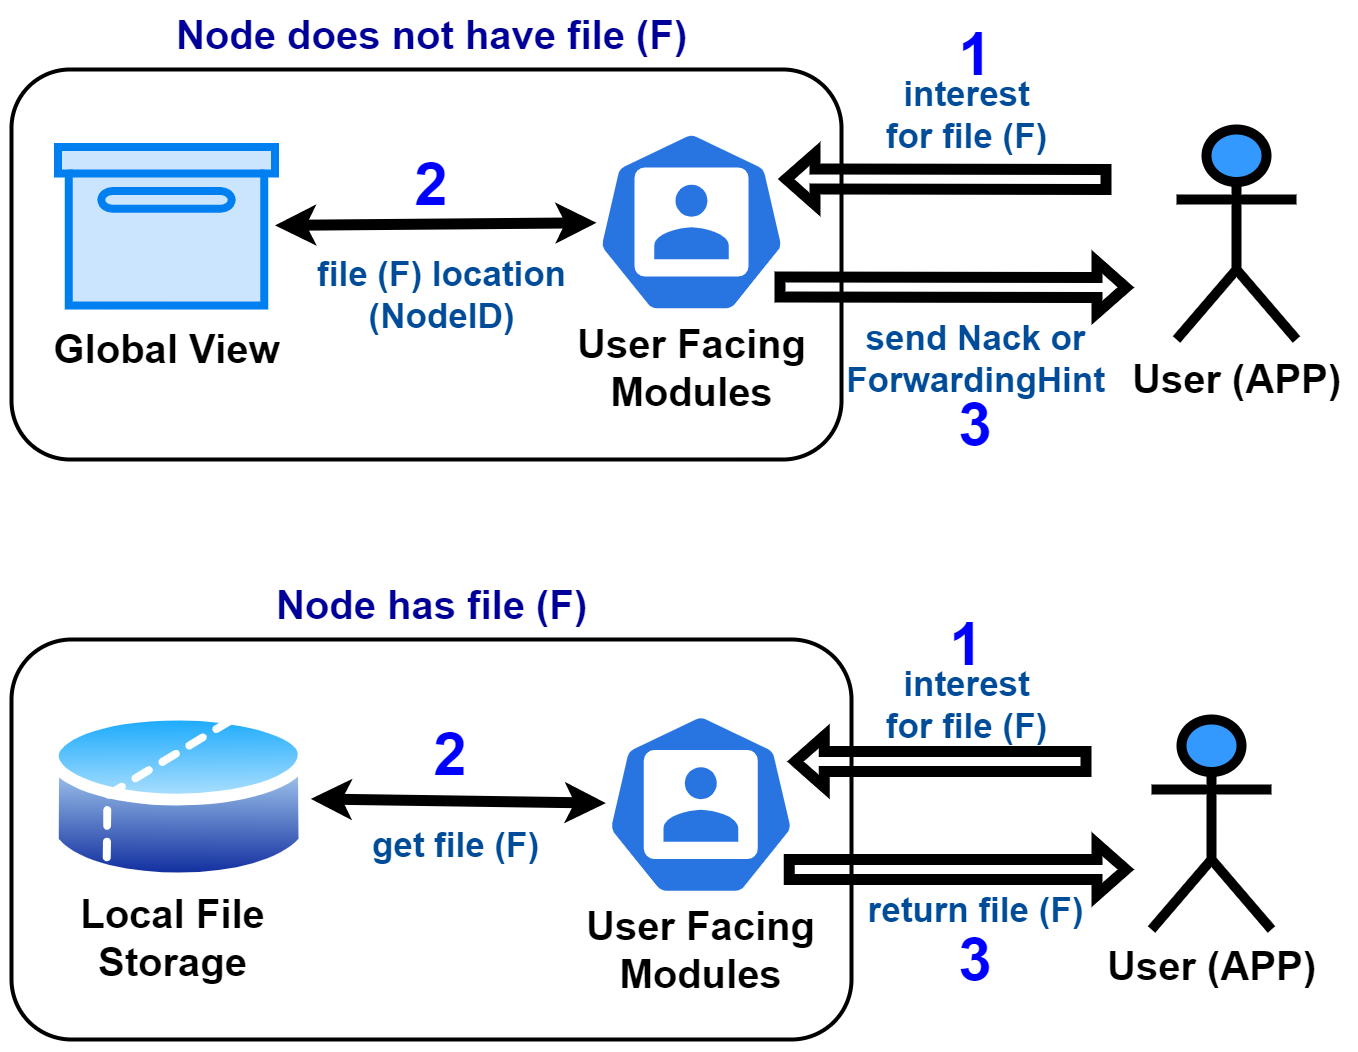
\includegraphics[width=\columnwidth]{visuals/fetch-sys.png}
    \caption{Module Interaction to Fulfill a User's Retrieval Requests}
    \label{fig:fetch-sys}
\end{figure}

Figure~\ref{fig:fetch-sys} shows two different situations. The Global View is used to indicate where the requested file is. After finding this information, the Hydra node responds to the user in the already-list 3 ways. In the case that the contacted node has the file, the local file storage is used to provide the file data. If a ForwardingHint is required, the node selects a random Hydra node that has the file and provides a unicast name (using the selected node's name) following the format /<node-name>/<hydra-prefix>/fetch/<file-name> for the user to use to fetch the file. Please note that this is the same format that a node uses to fetch a file from another node.
\subsection{Data Querying} \label{sec:data-query}


\todo[inline]{authentication needed}
\subsubsection{Scenario}
It has been two weeks since Alice from Subsection~\ref{sec:data-insert} published the processed (i.e. indexed) axolotl genome. In fact, she completely forgot that she did insert this data into the Hydra instance on FABRIC. When Alice received an error for trying to insert new data with the same name, she remembered about her forgotten inserted file. From Alice's perspective, having some way of querying to see what files are in Hydra and what file metadata is under a certain name is extremely useful. To satisfy this scenario, the following interactions are conducted.


\subsubsection{User-to-Node Interaction}
The process of how a user sends a query to a Hydra node can be described as a single Interest and a corresponding data packet. Any Hydra node can handle a query sent by the user. The naming of a query interest follows the format /<hydra-prefix>/query/<query-type>.


\subsubsection{Module Interaction}
\begin{figure}[!ht]
    \centering
    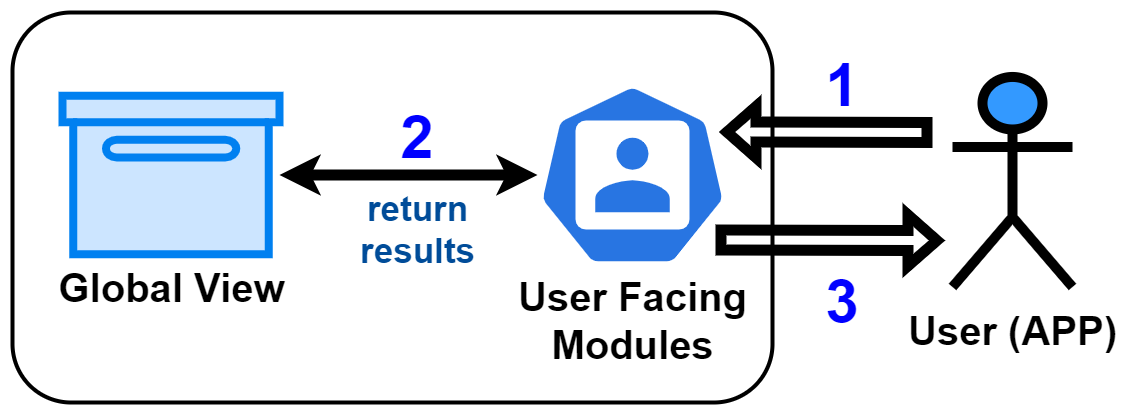
\includegraphics[width=\columnwidth]{visuals/query-sys.png}
    \caption{Module Interaction to Fulfill a User's Query Request}
    \label{fig:query-sys}
\end{figure}

The interest by the user gets processed in a simple way which is described by Figure~\ref{fig:query-sys}. The Hydra node simply checks the Global View for the query type information and returns it via a data packet.


\subsubsection{Types}
There are different query types that are defined. It is important to note that more queries can be added to better suit the environment, but also any queries can be disabled via Hydra's base policy. This gives Hydra instances more flexibility in what they want to expose to the users.

The query types are the following:
\begin{enumerate}
    \item /files: This allows users to see what files are within a Hydra instance. \todo[inline]{authentication?}
    \item /nodes: This allows users to see what nodes are part of a Hydra instance. \todo[inline]{why do users need to know this? I suggest you drop this. This might be a security problem. Yes, only super admins would have this power}
    \item /prefix/<prefix>: This allows users to search Hydra for files under a certain prefix.
    \item /file/<filename>: This allows users to see information about a certain file.
\end{enumerate}
\subsection{Data Deletion - Susmit} \label{sec:data-delete}


\subsubsection{Scenario} 
The same Alice found in Subsection~\ref{sec:data-insert} finds out that she made a grave mistake in pre-processing (i.e. indexing) the axolotl genome three weeks after she had inserted the data into Hydra. While Alice can wait a few more weeks to let the data naturally remove itself due to Hydra's base policy, she fears that anyone using her data before it gets removed will get false hope and possibly base future research on false data. This is a major concern for Clemson's Genomics and Bioinformatics facility as it can harmfully affect the facility's goal with using Hydra. Therefore, Alice needs a way to delete a file. To satisfy this scenario, the following interactions are conducted.


\subsubsection{User-to-Node Interaction} 
\begin{figure}[!ht]
    \centering
    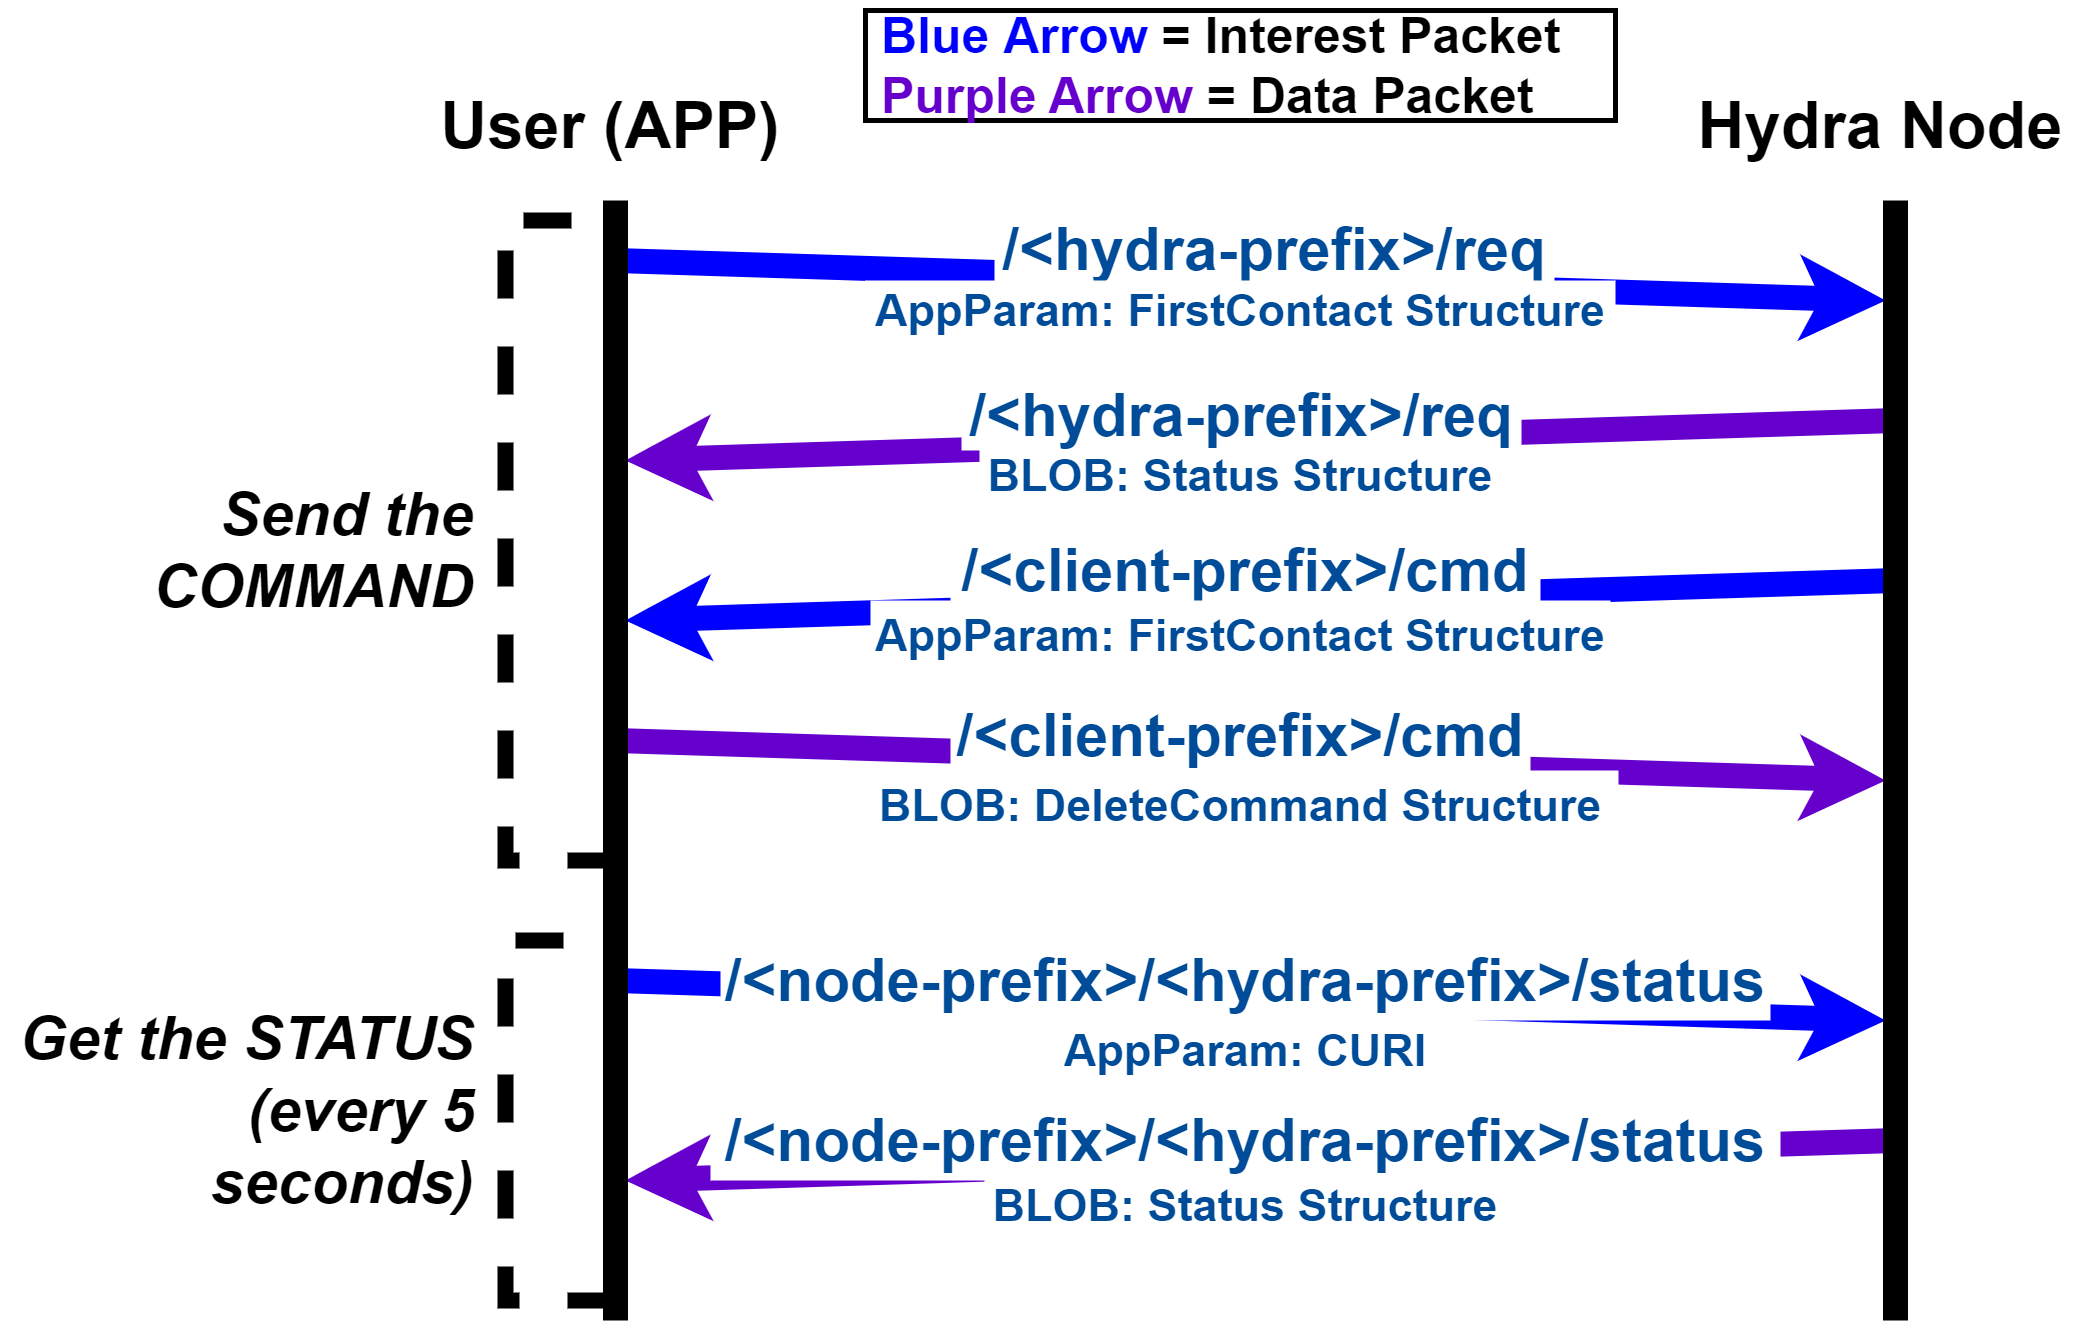
\includegraphics[width=\columnwidth]{visuals/delete-usr.png}
    \caption{NDN Interaction of a User and a Hydra Node During Deletion}
    \label{fig:delete-usr}
\end{figure}

The process of how a user will interact with a Hydra node via NDN is described in Figure~\ref{fig:delete-usr} and shares great similarities with data insertion. Any Hydra node can be contacted by the user for data deletion, and this interaction can be summarized as a PubSub-like interaction: it uses a notification interest with a component /notify and a data retrieval interest with a component /msg.

This interaction between user (A) and node (X) goes as follows:
\begin{enumerate}
    \item User (A) will send a interest notification using the prefix /<hydra-prefix/delete, announcing that it has a command for any Hydra node to process.
    \item Upon hearing this, node (X) will send an interest to fetch this command using user (A)'s prefix (stated in user (A)'s FirstContact structure found in the interest notification's app parameters).
    \item Node (X) will process this command and than send a notification interest stating that the command that user (A) sent has a updated status.
    \item User (A) can then fetch the status of the command using node (X)'s prefix (stated in node (X)'s FirstContact structure found in a previous interest).
\end{enumerate}

The exact same key points found in Subsection~\ref{sec:data-insert} for User-to-Node interaction applies for this process as well.


\subsubsection{Module Interaction} 
\begin{figure}[!ht]
    \centering
    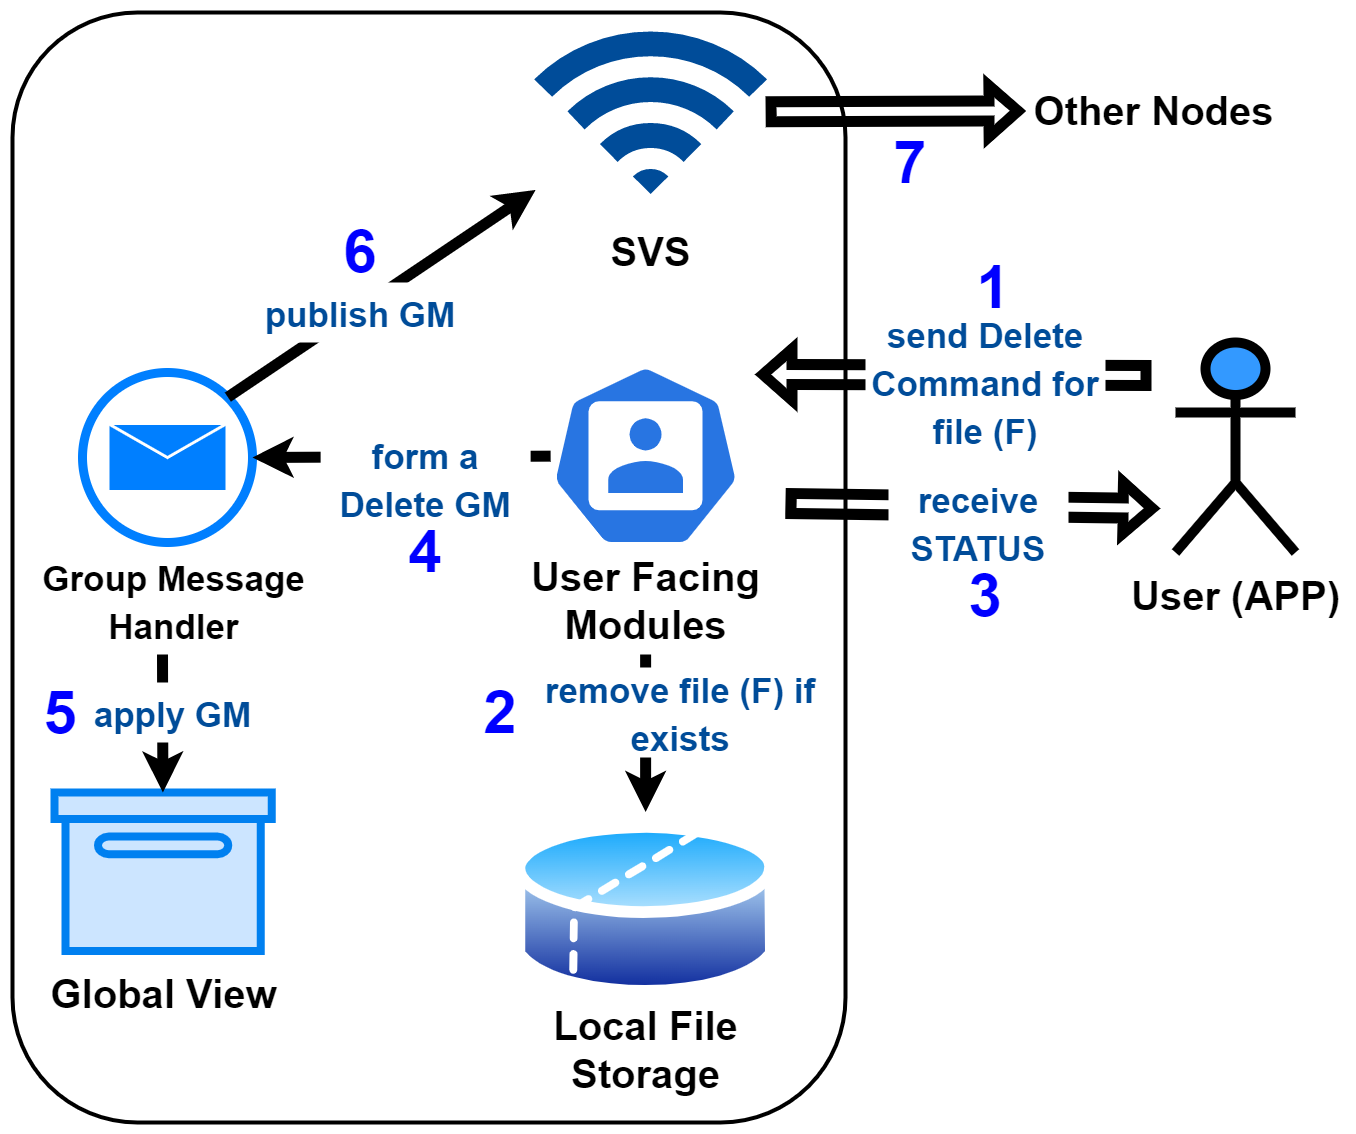
\includegraphics[width=\columnwidth]{visuals/delete-sys.png}
    \caption{Module Interaction to Fulfill a User's Deletion Command}
    \label{fig:delete-sys}
\end{figure}

The User-to-Node interaction leads to Module interaction where a Hydra node will act out the given command. As seen in Figure~\ref{fig:delete-sys}, when node (X) receives a Deletion command for file (F) from user (A):
\begin{enumerate}
    \item Node (X) properly authenticates the command.
    \item Node (X) deletes any local copies of file (F).
    \item Node (X) updates the status for user (A) allowing user (A) to go offline.
    \item Node (X) forms a Delete GM which includes the name of file (F).
    \item Node (X) applies this GM to its Global View: all file (F) information is removed.
    \item Node (X) publishes this GM using SVS, our distributed synchronization protocol.
\end{enumerate}

Every node will receive the Delete GM. When node (Y) receives the Delete GM sent by node (X) containing file (F)'s name:
\begin{enumerate}
    \item Node (Y) deletes any local copies of file (F).
    \item Node (Y) applies the GM to its Global View: all file (F) information is removed.
\end{enumerate}


\subsubsection{Data Structure Formats} 
There are several structures that are used for the entire data deletion process. For the group message structures used in Module interaction, please refer back to Section~\ref{sec:group-messages}. In addition, most of the other structures are the same ones described in Subsection~\ref{sec:data-insert}. The only missing structure is DeleteCommand which holds the filename of the desired-to-be-removed file.